\section{Paper 2 highlights: What would other emergency stroke teams do? Using explainable machine learning to understand variation in thrombolysis practice.\cite{pearn_what_2023}}\label{sec:paper_2}

\subsection{Objective}

To understand, using explainable machine learning, between-hospital variation in thrombolysis use among emergency stroke admissions in England and Wales.

\subsection{Methods overview}


Data were retrieved for 246,676 emergency stroke admissions to acute stroke teams in England and Wales for the years 2016–2018, obtained from the Sentinel Stroke National Audit Programme (SSNAP). Data fields were provided for the hyper-acute phase of the stroke pathway, up to and including our target feature: receive thrombolysis. Of these patients, 88,928 were used in this modelling study: arrived within 4 hours of known stroke onset, had onset out of hospital, had an arrival to scan time recorded, and attended a hospital with at least 300 emergency stroke admissions and at least 10 thrombolysis procedures. A 4 hours onset-to-arrival cut-off was used to allow for 30 minutes for scan and thrombolysis to be within the allowed 4.5 onset-to-thrombolysis time. The data included 132 acute stroke hospitals. We trained a machine learning model (XGBoost\cite{chen_xgboost_2016}) to learn which patients would receive thrombolysis at each stroke team. Shapley (SHAP) values were calculated for each prediction, providing estimates of how patient features, and hospital identity, influence the odds of receiving thrombolysis \cite{lundberg_unified_2017}.

Code, and full results, for the machine learning work may be found at 
 \url{https://samuel-book.github.io/samuel_shap_paper_1}

\subsection{Key results}

\subsection{Feature selection}

The best model with 1, 2, 5, 10, 25 \& all 83 original features had ROC AUCs of 0.716, 0.792, 0.893, 0.919, 0.923 \& 0.922. We selected 10 features for all subsequent work, which were:

\begin{itemize}
    % codeing of data (e.g. 0/1 or yes/no not needed here)
    \item \emph{Arrival-to-scan time}: Time from arrival at hospital to scan (minutes)
    \item \emph{Infarction}: Stroke type (infarction/haemorrhage)
    \item \emph{Stroke severity}: National Institutes of Health Stroke Scale (NIHSS) score on arrival
    \item \emph{Precise onset time}: Onset time (\textit{precise}, or \textit{best estimate})
    \item \emph{Prior disability level}: Estimated mRS score prior to stroke
    \item \emph{Stroke team}: Stroke team attended (hospital identifier)
    \item \emph{Use of atrial fibrillation (AF) anticoagulants}: Use of prior anticoagulants for atrial fibrillation.
    \item \emph{Onset-to-arrival time}: Time from onset of stroke to arrival at hospital (minutes)
    \item \emph{Onset during sleep}: Did stroke occur in sleep? (1 = Yes, 0 = No)
    \item \emph{Age}: Age (as midpoint of 5 year age bands)
\end{itemize}

Correlations between the 10 features were measured using coefficients of determination (r-squared). All r-squared were less than 0.05 except (a) age and prior disability level (r-squared 0.146), and (b) onset during sleep and precise onset time (r-squared 0.078).

\subsubsection{Model accuracy}

Model accuracy was measured using stratified 5-fold cross validation. Overall accuracy was 85.0\% (83.9\% sensitivity and specificity could be achieved simultaneously). Receiver Operating Characteristic Area Under Curve (ROC-AUC) was 0.918. The model predicted hospital thrombolysis use at each hospital with very good accuracy (r-squared = 0.977, with a mean absolute error of 1.1 percentage points).

\subsubsection{Individual patient prediction}

SHAP values are calculated as log-odds as these are additive; the final model prediction, as log odds, is the sum of the individual feature SHAP values and the base SHAP value which is common to all predictions. For illustrative purposes, probabilities may also be used. Figure \ref{fig:waterfall} shows SHAP values for an individual patient prediction. illustrated as a \textit{waterfall} plot, shown as either log odds or probabilities.


\begin{figure}
    \centering
    \begin{subfigure}[b]{0.48\textwidth}
        \centering
        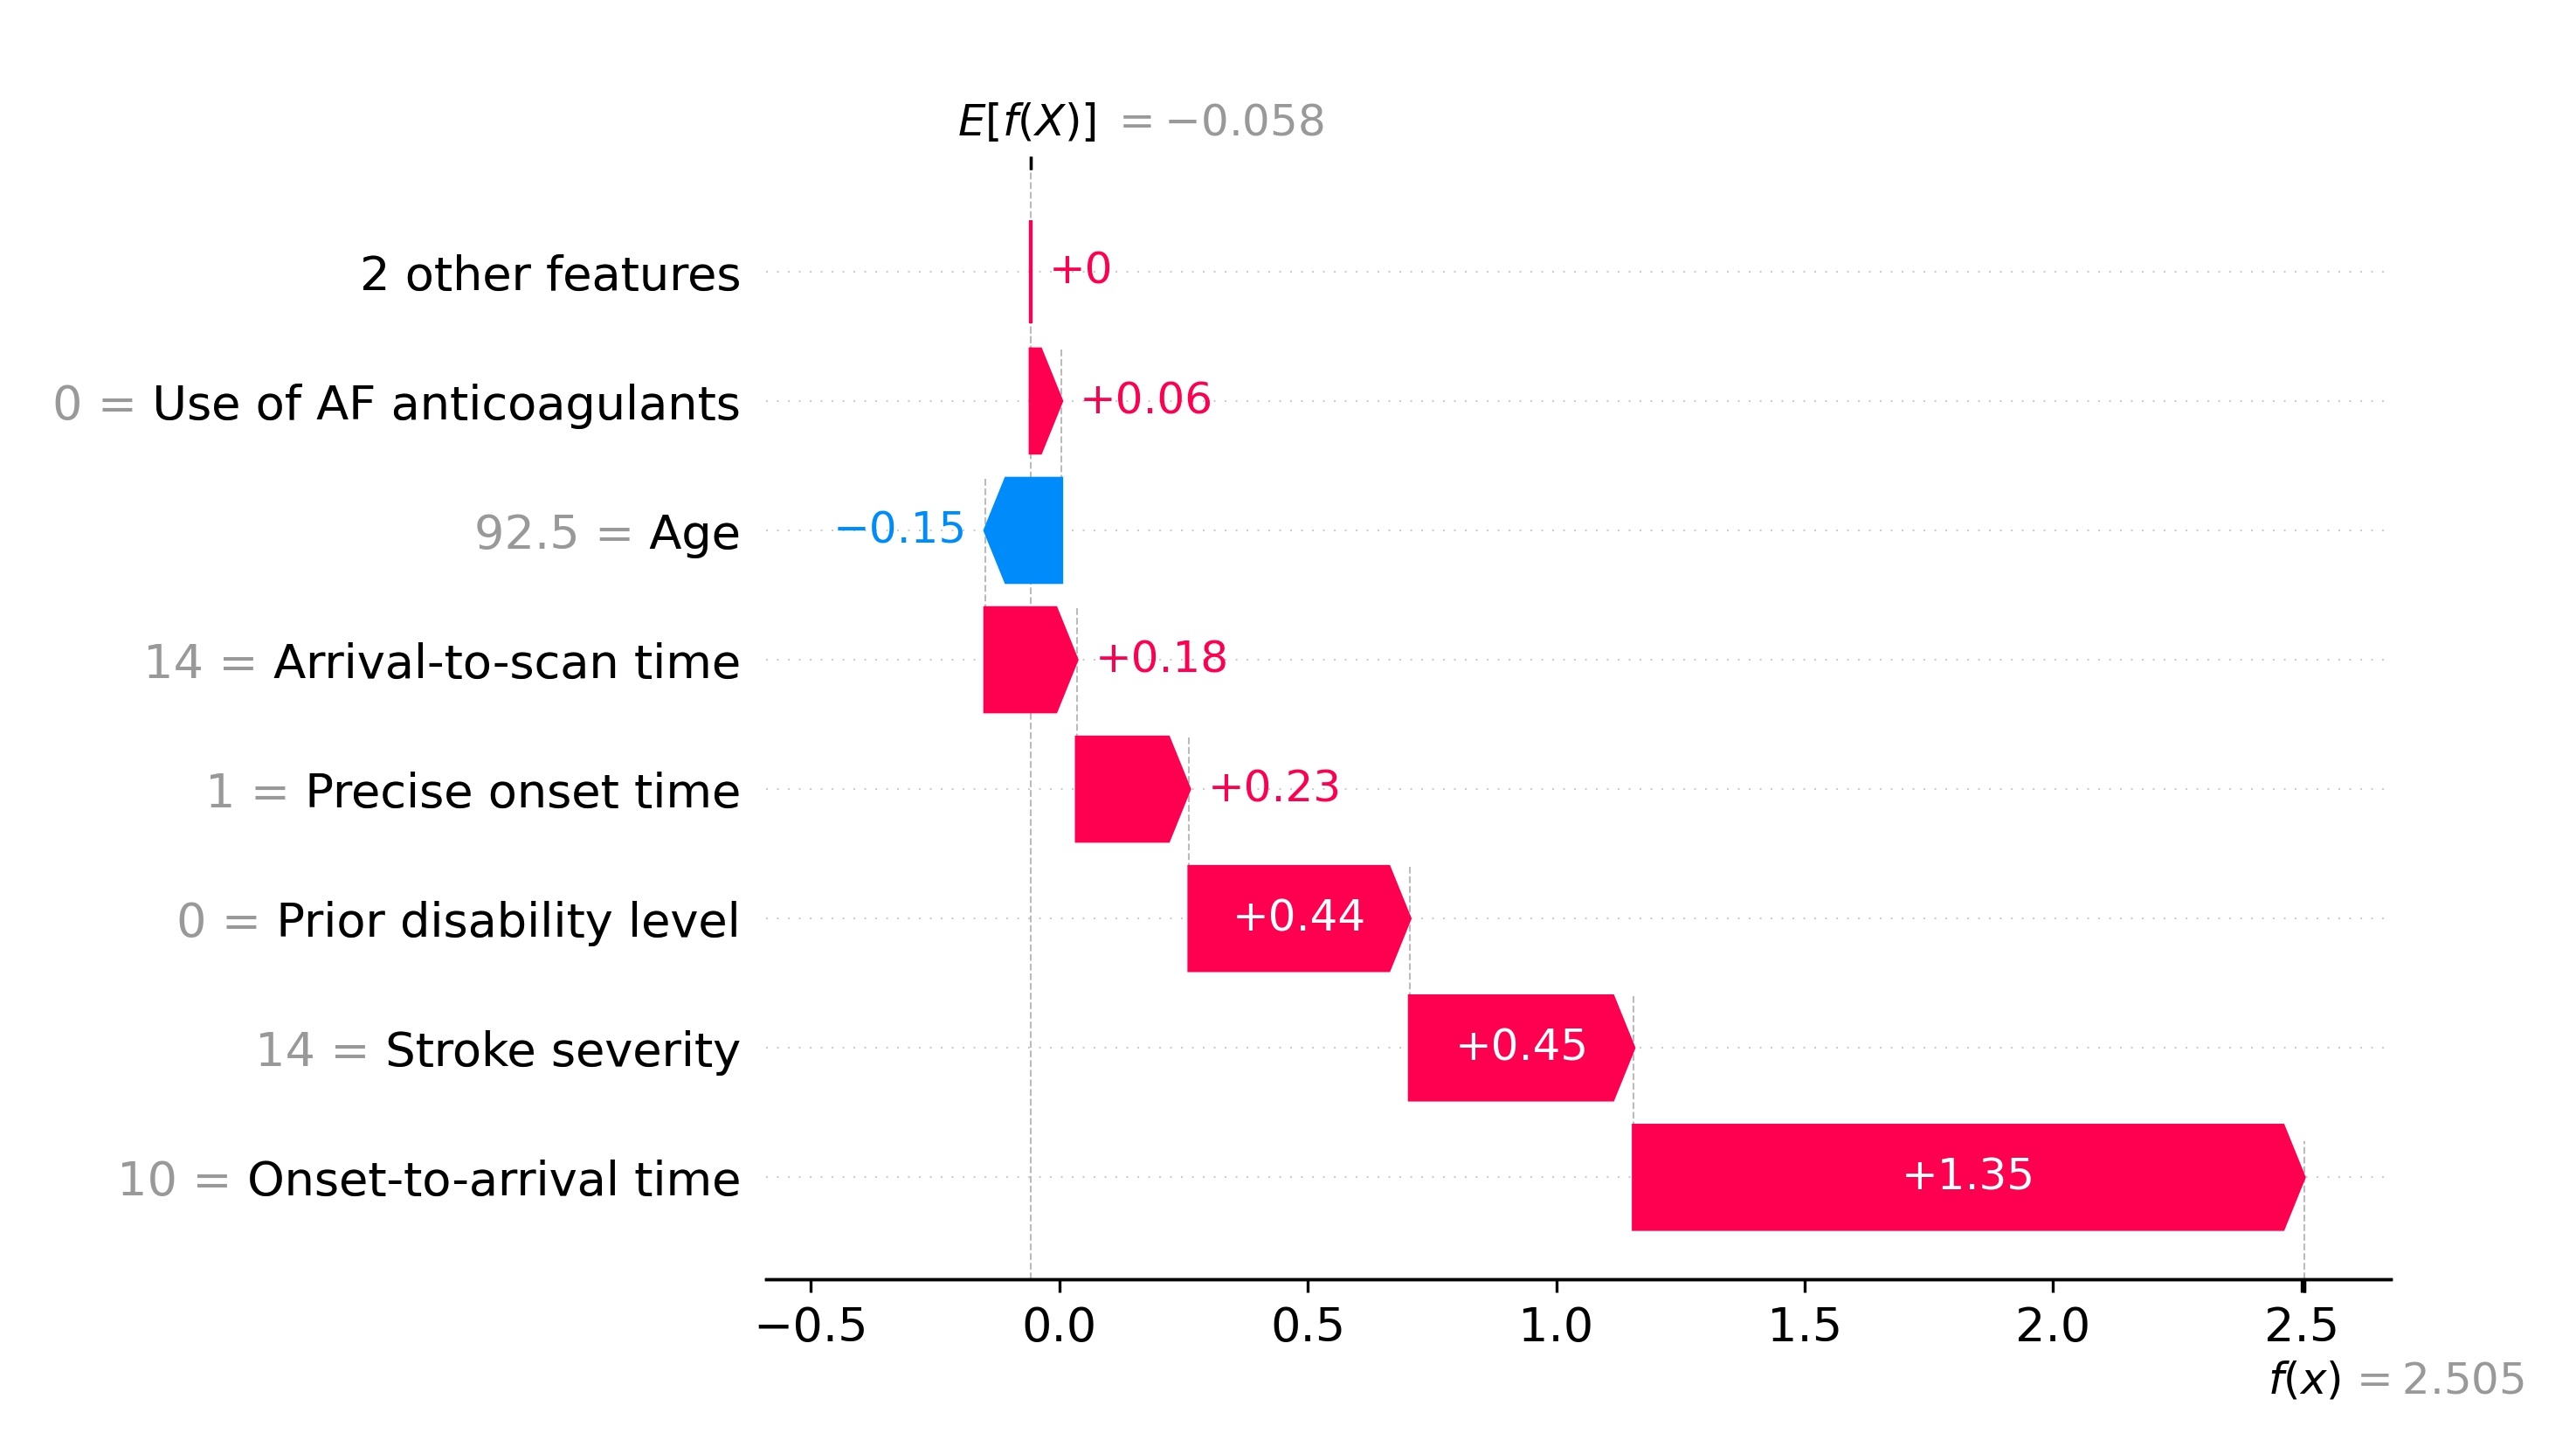
\includegraphics[width=\textwidth]{images/p2_waterfall_odds.jpg}
        \caption{log odds}
        \label{fig:waterfall_subfig1}
    \end{subfigure}
    \hfill
    \begin{subfigure}[b]{0.48\textwidth}
        \centering
        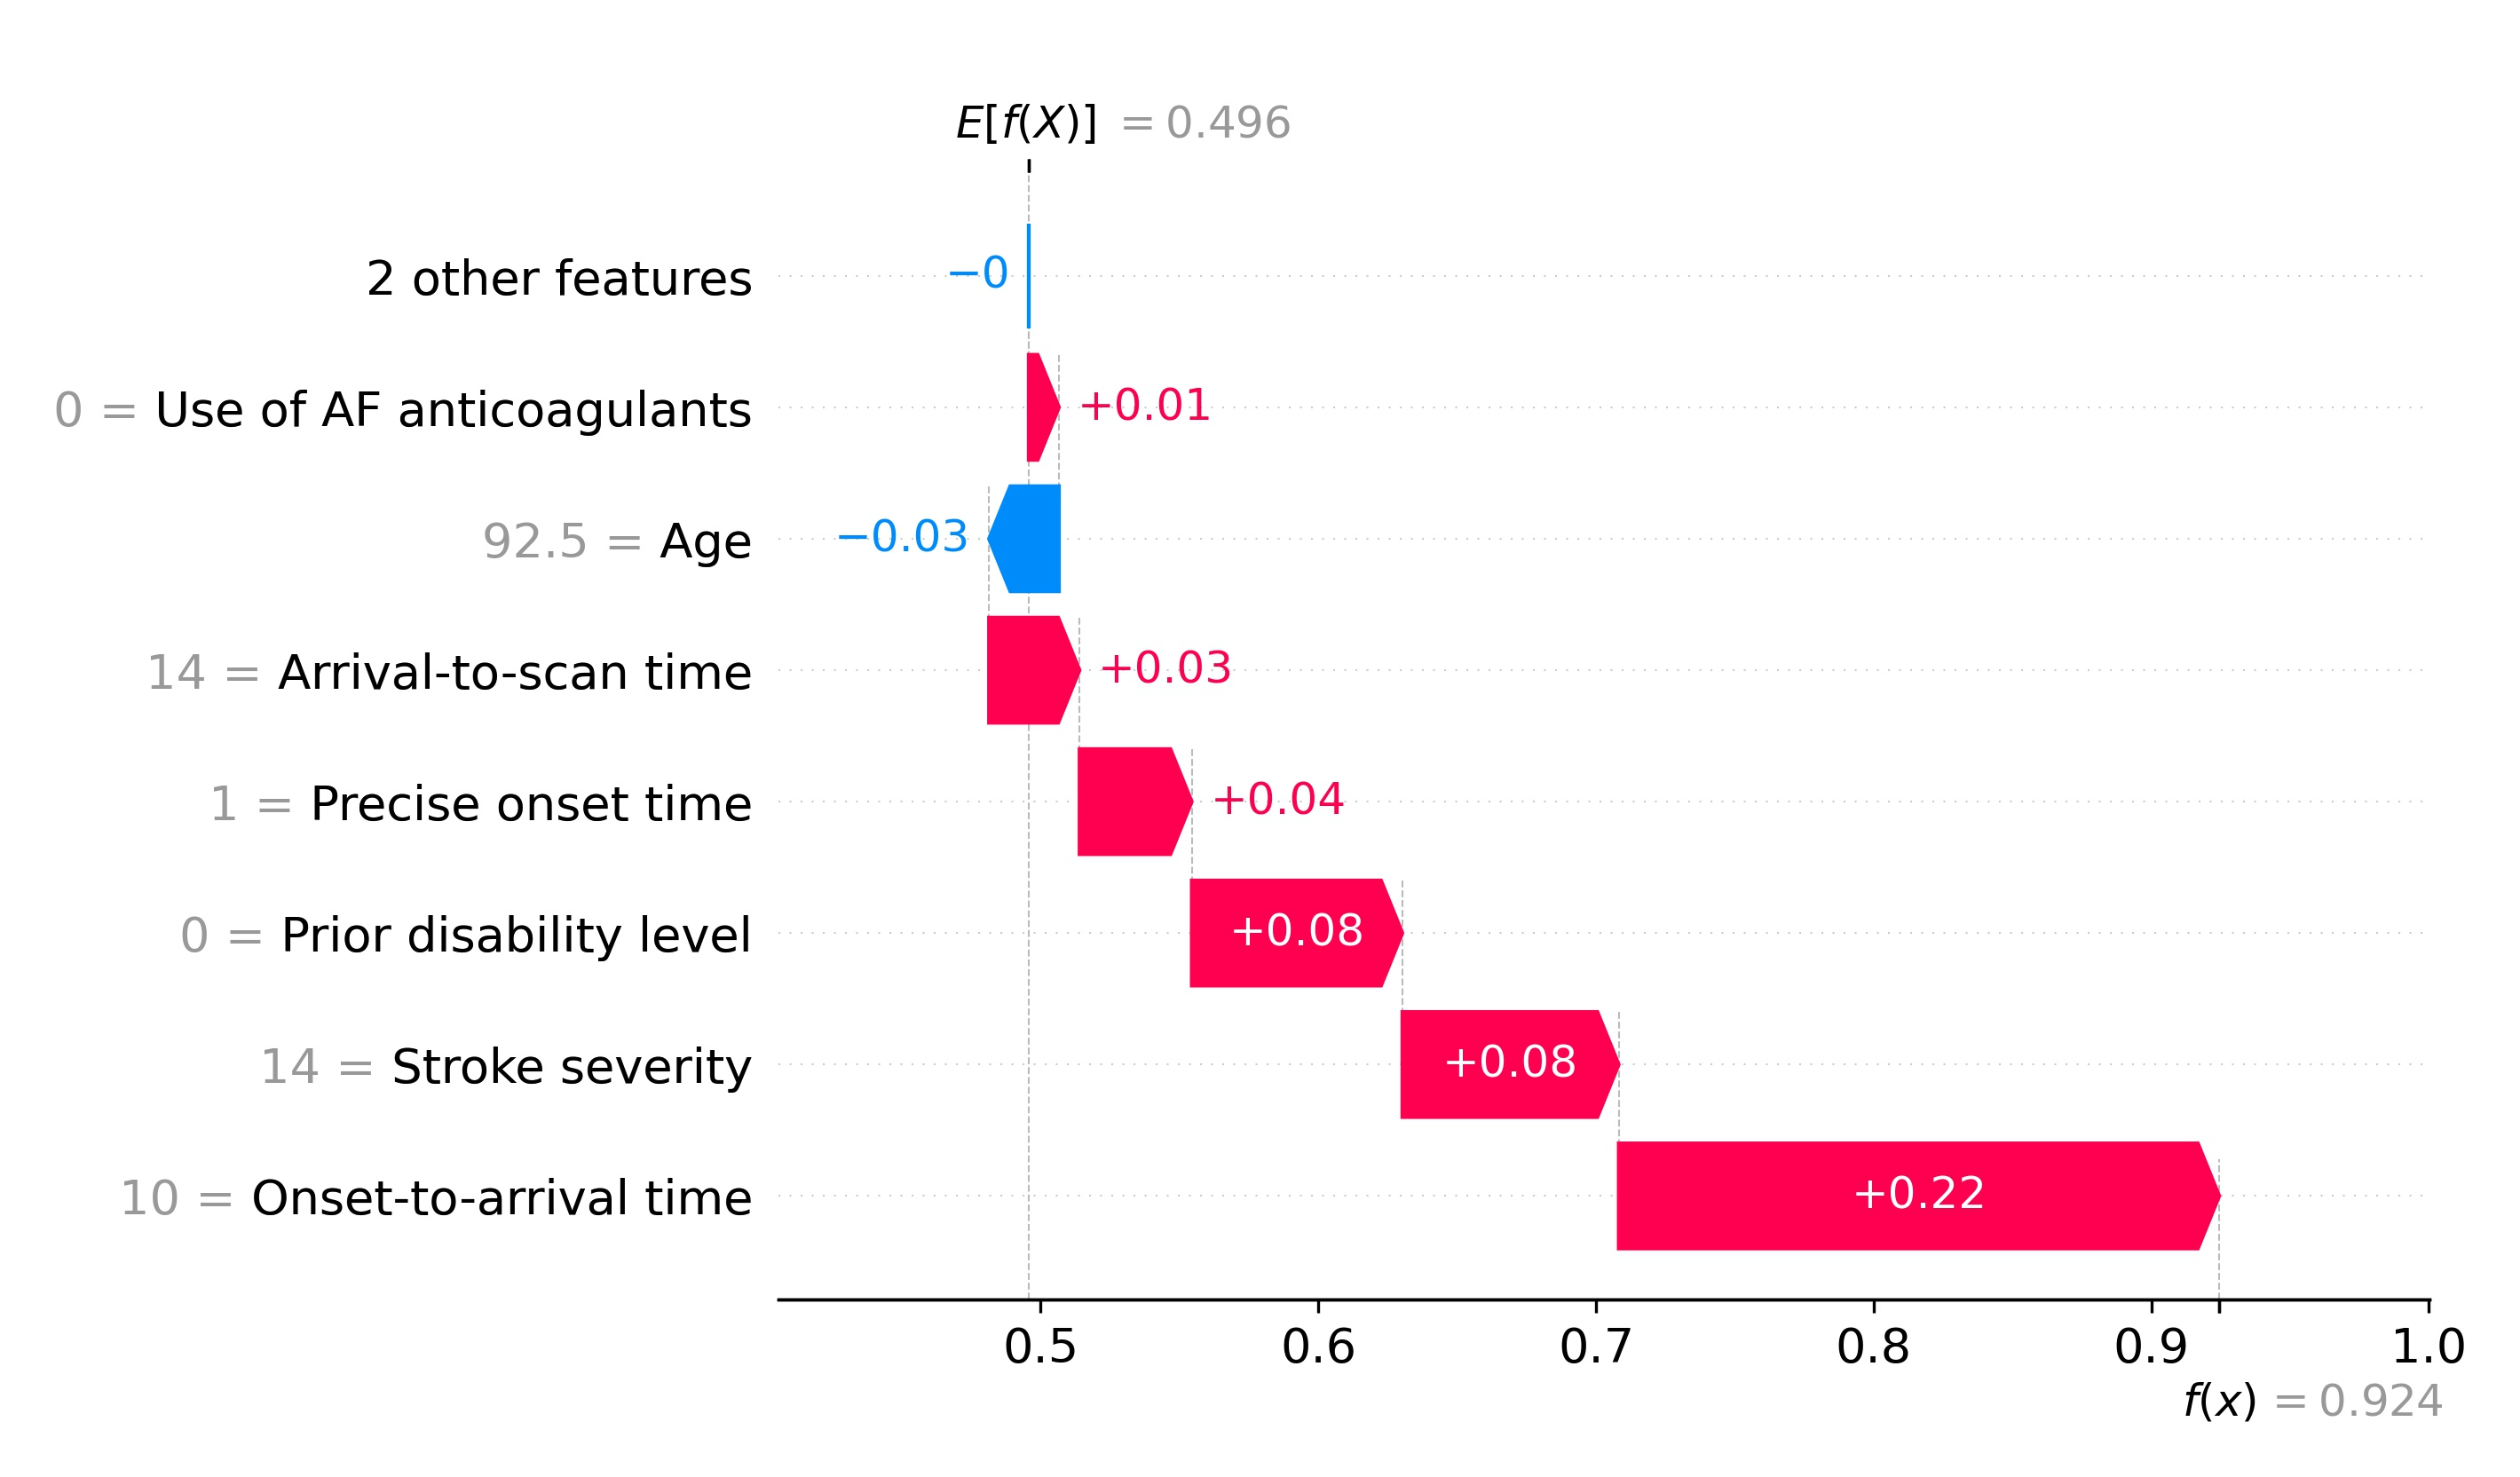
\includegraphics[width=\textwidth]{images/p2_waterfall_probs.jpg}
        \caption{probabilities}
        \label{fig:waterfall_subfig2}
    \end{subfigure}
    \caption{A waterfall plot for an example patient with model prediction and SHAP values expressed either as log odds (left) or probabilities (right). Predictions start with a base value (common to all predictions) of -0.058 log odds or 49.6\% probability of receiving thrombolysis. The individual patient values then contribute to a final prediction of 2.505 log odds or 92.4\% probability of receiving thrombolysis. The most influential features, all increasing the odds of receiving thrombolysis were no prior disability, a severe stroke (NIHSS 14), and 10 minutes onset-to-arrival time.}
    \label{fig:waterfall}
\end{figure}

\subsubsection{Global patterns of patient factors affecting use of thrombolysis}

Global patterns of how feature values affect the odds of receiving thrombolysis are constructed by combining all individual patient prediction SHAP values for each feature. 

Figure \ref{fig:global_shap} shows the relationship between patient characteristics and the log odds of receiving thrombolysis. Key observations are (with SHAP influence converted from log-odds to odds):

\begin{itemize}
    \item \emph{Stroke type}: The SHAP values for stroke type show that the model effectively eliminated any probability of receiving thrombolysis for non-ischaemic (haemorrhagic) stroke.
    \item \emph{Arrival-to-scan time}: The odds of receiving thrombolysis reduced by about 9-fold over the first 120 minutes of arrival-to-scan time.
    \item \emph{Stroke severity (NIHSS)}: The odds of receiving thrombolysis were lowest at NIHSS 0, increased and peaked at NIHSS 15-25, and then fell again with higher stroke severity (NIHSS above 25). The difference between minimum odds (at NIHSS 0) and maximum odds (at 15-25) of receiving thrombolysis was 25 to 30-fold.
    \item \emph{Stroke onset time type (precise vs. estimated)}: The odds of receiving thrombolysis were about 3-fold greater for precise onset time than estimated onset time.
    \item \emph{Disability level (mRS) before stroke}: The odds of receiving thrombolysis fell about 6-fold between mRS 0 and 5.
    \item \emph{Use of AF anticoagulants}: The odds of receiving thrombolysis were about 5-fold greater for no use.
    \item \emph{Onset-to-arrival time}: The odds of receiving thrombolysis were similar below 120 minutes, then fell about 3-fold between 120 and 240 minutes.
    \item \emph{Age}: The odds of receiving thrombolysis were similar below 80 years old, then fell about 2-fold between 80 and 110 years old.    
    \item \emph{Onset during sleep}: The odds of receiving thrombolysis were about 4-fold lower for onset during sleep.
\end{itemize}

\begin{figure}
    \centering
    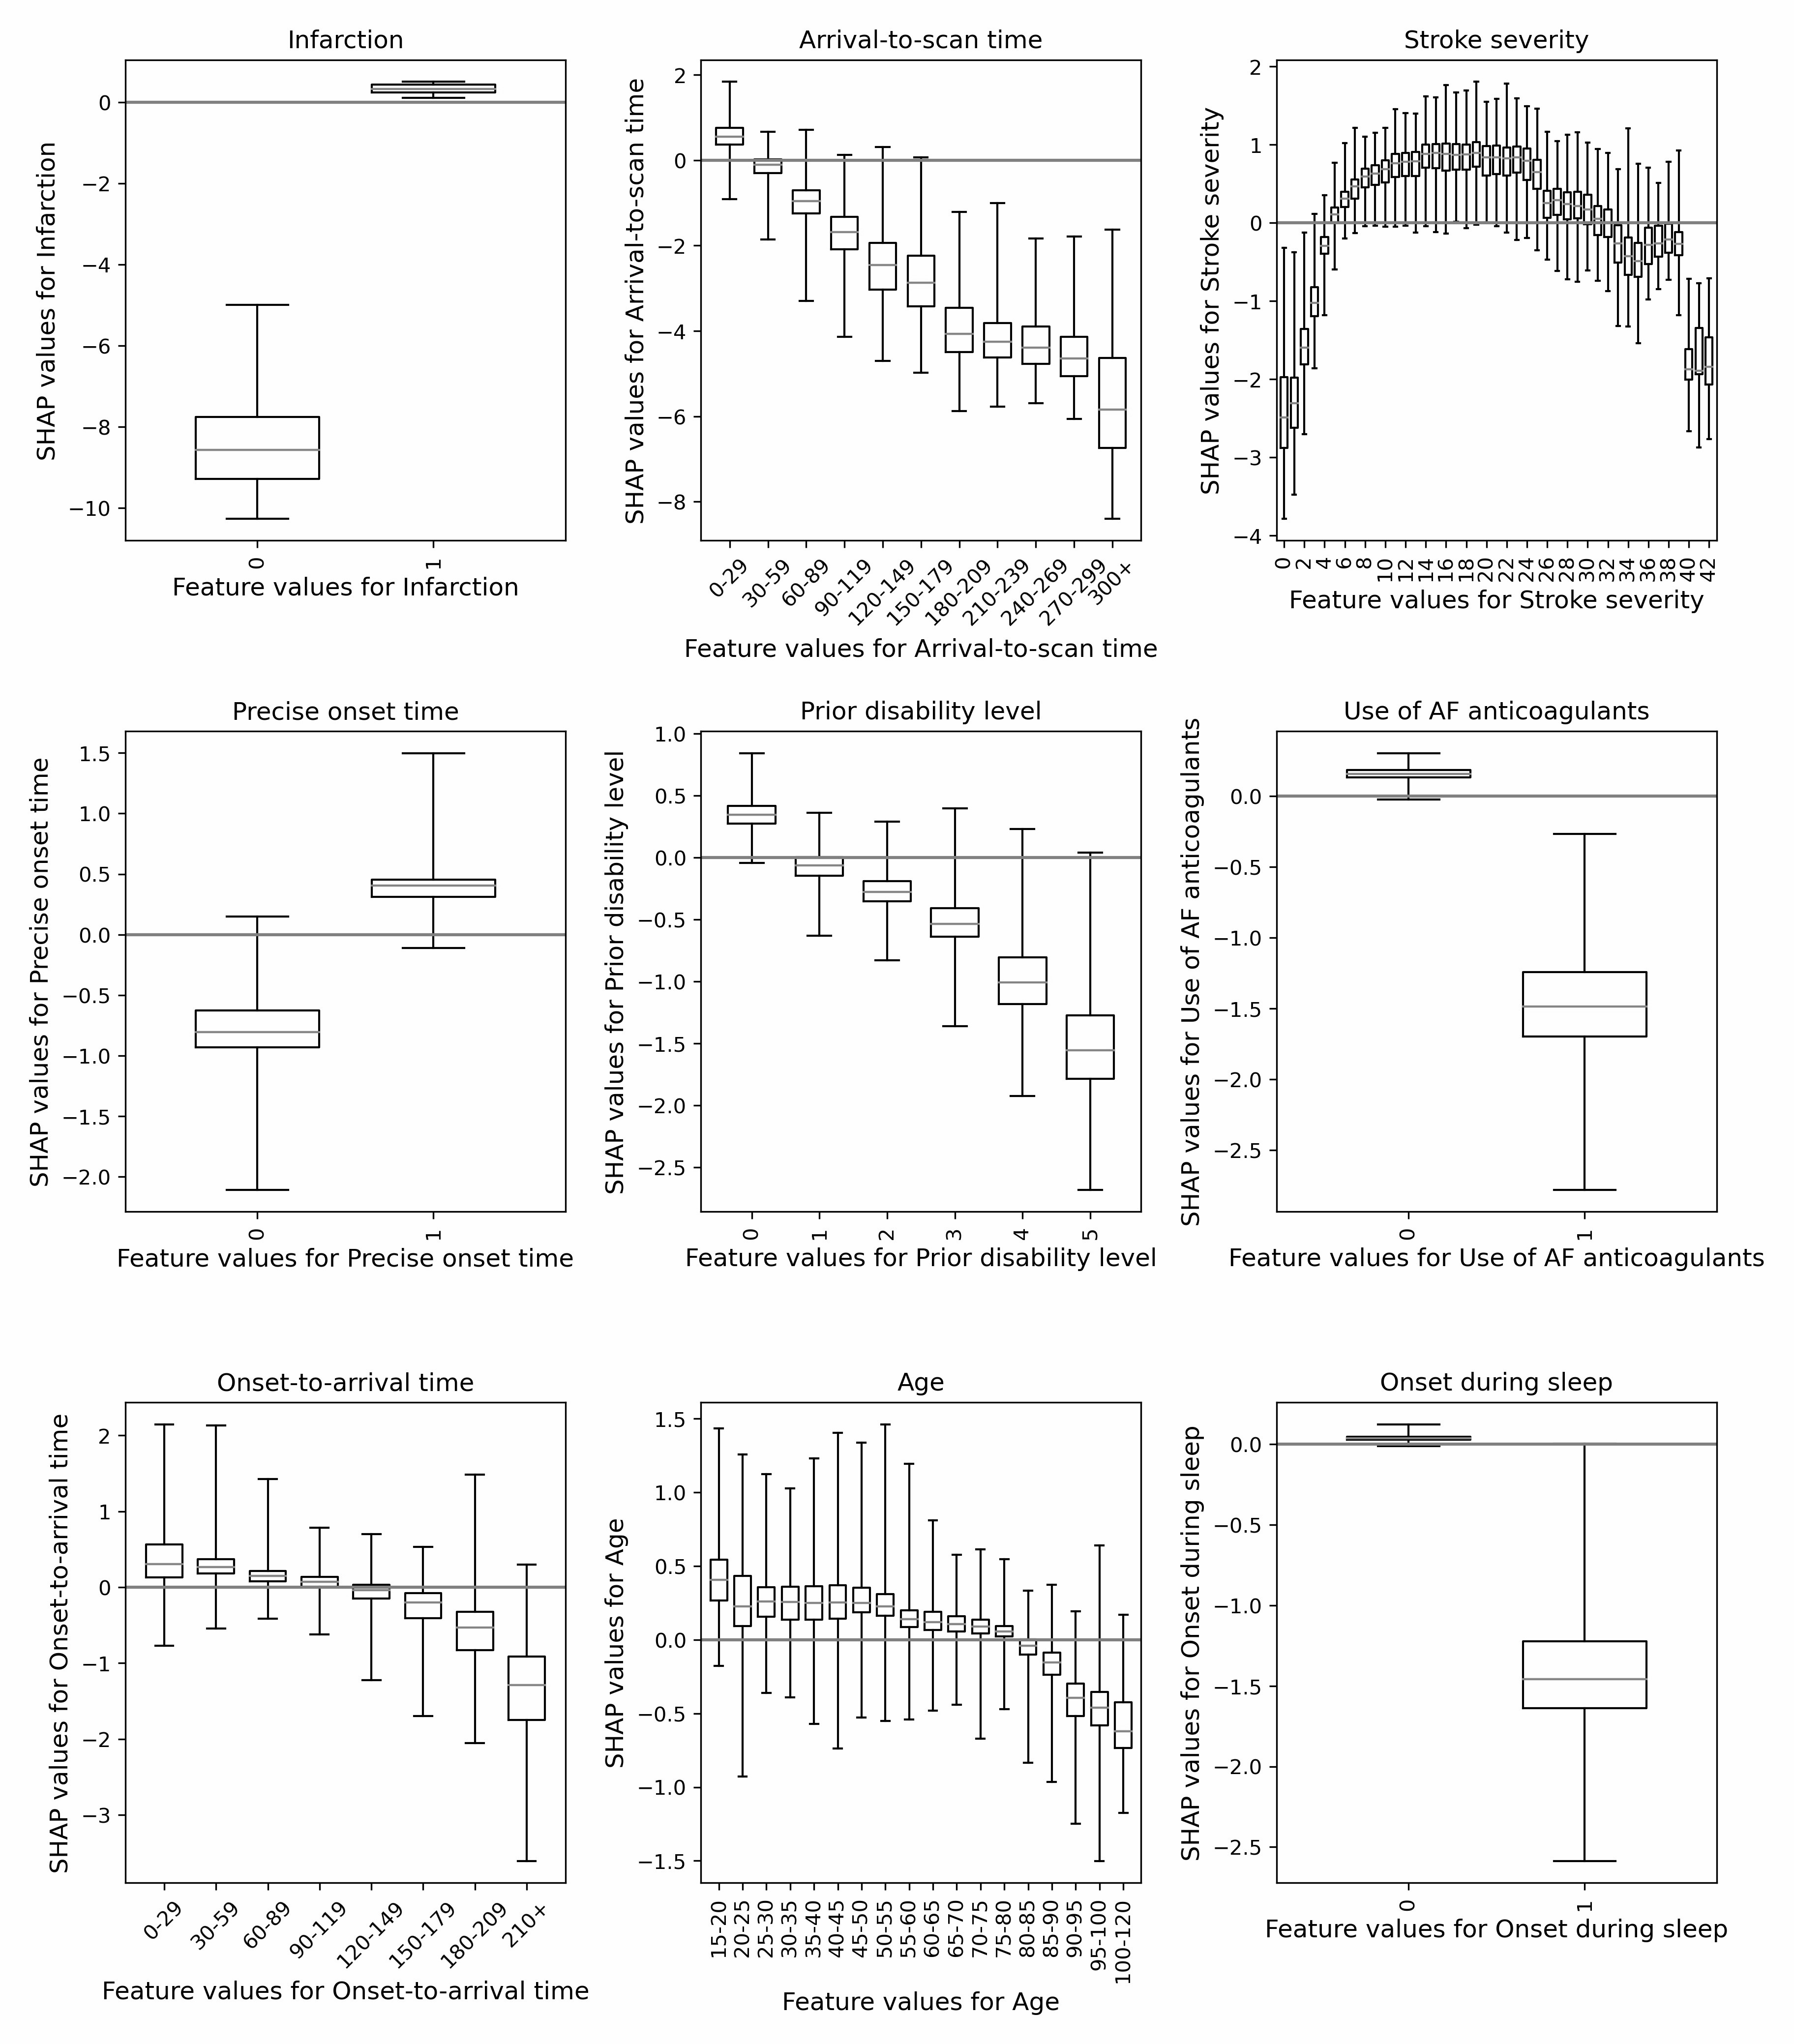
\includegraphics[width=1\linewidth]{images/p2_patient_shap.jpg}
    \caption{Box plots showing the relationship between SHAP values and feature values. Box plots show inter-quartile range (box), median (mid-line in box), and range (whiskers). The plots are ordered in ranked feature importance (using the mean absolute SHAP value across all instances).}
    \label{fig:global_shap}
\end{figure}

\subsubsection{How hospital attended affects the odds of receiving thrombolysis}

Figure \ref{fig:hospital_shap} shows the distribution of SHAP values for hospital attended. The hospital SHAP value isolates the affect that attending any given hospital has on the odds of receiving thrombolysis. There was a 13-fold difference in odds of receiving thrombolysis between hospitals.

\begin{figure}
    \centering
    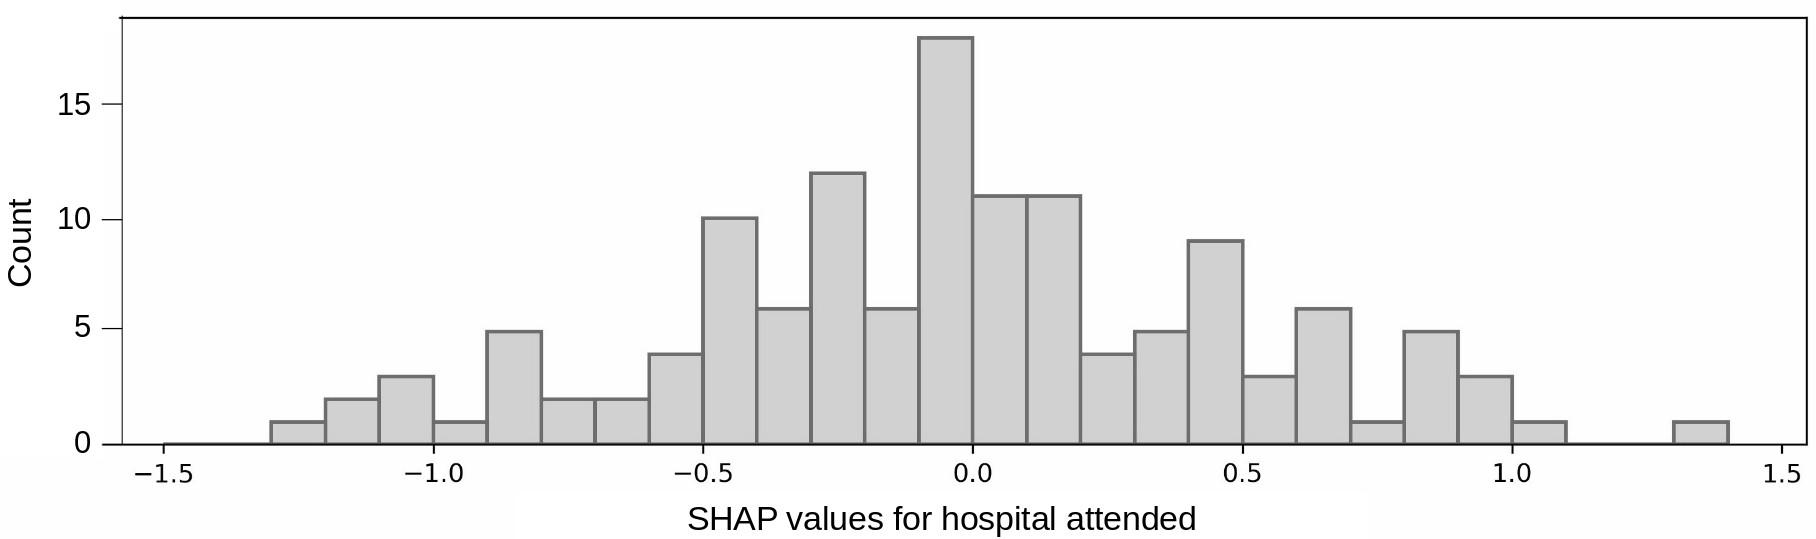
\includegraphics[width=1\linewidth]{images/p2_hosp_shap.jpg}
    \caption{Histogram showing the frequency of SHAP values for the hospital attended.}
    \label{fig:hospital_shap}
\end{figure}

Overall we found 36\% of the variance in observed between-hospital thrombolysis use can be explained by the patient population characteristics (age, stroke severity, prior disability, onset-to-arrival time, stroke type, type of onset time, anticoagulants, and onset during sleep), 74\% can be explained by hospital identity and processes (arrival-to-scan time, and hospital attended), and that 95\% can be explained by the combined information from both the patient population and hospital identity and processes.

We compared expected thrombolysis use in subgroups of patients. This is not included in this synopsis, as it is more clearly demonstrated in the \textit{prototype patients} analysis in section \ref{sec:paper_5}. In summary we found all stroke teams were very likely to give thrombolysis to \textit{ideal candidates} for thrombolysis, but they varied in their likelihood to give thrombolysis to patients with non-ideal characteristics such as mild stroke, imprecisely known onset time, or patients with pre-stroke disability. 

\subsection{Conclusions}

Using explainable machine learning on a large national stroke registry dataset, we have identified how patient features and hospital attended influence decisions to treat with thrombolysis. We showed that the majority of the between-hospital variation in thrombolysis use in England and Wales, for patients arriving with time to thrombolyse, is explained by differences between in-hospital processes and differences in attitudes to eligibility for thrombolysis.